\documentclass[11pt]{article}
\usepackage[utf8]{inputenc}
\usepackage[T1]{fontenc}
\usepackage{amsmath}
\usepackage{amsfonts}
\usepackage{amssymb}
\usepackage[version=4]{mhchem}
\usepackage{stmaryrd}
\usepackage{hyperref}
\hypersetup{colorlinks=true, linkcolor=blue, filecolor=magenta, urlcolor=cyan,}
\urlstyle{same}
\usepackage{graphicx}
\usepackage[export]{adjustbox}
\graphicspath{ {./images/} }

\begin{document}
Historical Returns of Co-investment

\section*{Evidence on the Performance of Co-investments}
Evidence on the performance of co-investments is mixed and varies by the study and the data set reviewed. Co-investing is often pitched to LPs as a way to obtain access to private equity with a known GP and to reduce costs when the LPs are waiting for other opportunities in which to deploy funds. However, when the GP offers lower-cost access to one or more of their portfolio companies, it may create concerns on the part of the LP regarding the quality of the opportunity they are being offered. In fact, a study by Fang, Ivashina, and Lerner (2015) ${ }^{1}$ Fang, L., V. Ivashina, and J. Lerner (April 2015), The Disintermediation of Financial Markets: Direct Investing in Private Equity, Journal of Financial Economics 116 (1): 160-78. addresses this important issue regarding the quality of co-investment deals. These researchers find that co-investments have underperformed the corresponding funds. Specifically, the study finds:

\begin{itemize}
  \item The evidence of underperformance of co-investments may be associated with the higher risk of such deals.
  \item Importantly, the evidence found a sharp contrast between the performance of "solo" deals, in which institutional investors source direct investments independently from GPs, and that of co-investment deals. This points to a potential conflict of interest and a potential principal-agent problem because GPs may selectively offer deals to their LPs.
  \item Crucially, however, the results of the study are based on deals in which LPs took no active role in sourcing opportunities and only co-invested in deals offered to them, apparently based on deal size. (The deals were nearly five times larger than the funds' average deals.)
\end{itemize}

The specific modus operandi that co-investments are offered only by GPs to their LPs is not necessarily representative. ${ }^{2}$ Ibid. Practitioners point out that it is important that LPs generate their co-investment deal flows like any other direct investor would. ${ }^{3} \mathrm{Ibid}$. The PE market environment has a strong influence on the types of industries from which these co-investment opportunities are sourced and on the timing of the flows. Co-investment opportunities emerge particularly in periods when deal flow for larger investments is good but fundraising is difficult. In this situation, and also when funds do not wish to be overexposed to one particularly large deal, GPs are likely to turn to their LPs and propose a co-investment.

Braun et al. (2016) ${ }^{4}$ Ibid criticized Fang et al. (2015) for using data collected from just 7 LPs who participated in both solo and co-investments deals, which provided 103 co-investments observations. Some suggested that the data set may be limited in scale and not be representative of co-investment performance. ${ }^{5}$ Braun, Reiner, Tim Jenkinson, and Christoph Schemmerl, Adverse Selection and the Performance of Private Equity Co-Investments (December 14, 2018), \href{https://ssrn.com/abstract=2871458}{https://ssrn.com/abstract=2871458} or \href{http://dx.doi.org/10.2139/ssrn}{http://dx.doi.org/10.2139/ssrn}. 2871458 Braun et al. (2016) used a larger data set, which provided 365 observations of buyout co-investments and 615 venture capital co-investments over a period of 32 years, from 1978 to 2010.

In contrast to the conclusions of Fang et al. (2015), Braun finds:

\begin{itemize}
  \item Buyout co-investments and venture capital co-investments outperform their corresponding funds.
  \item Co-investments generally have lower costs to investors compared to funds.
  \item There is no evidence of GPs offering LPs lower-quality deals since co-investment deals did not underperform against their corresponding funds. Instead, Braun et al. noted that GPs may use co-investments to develop stronger relationship with existing or target LPs before their next fundraising. Furthermore, the longterm economic value of a GP is driven by their ability to raise future funds (Chung, Sensoy, Stern, and Weisbach 2012). ${ }^{6}$ Ji-Woong Chung, Berk A. Sensoy, Léa Stern, and Michael Weisbach (2012), Pay for Performance from Future Fund Flows: The Case of Private Equity. in Review of Financial Studies 25 (11): $3259-$ 3304 .
\end{itemize}

The findings of Braun et al. (2016) echo the results from a GP survey conducted by Preqin (2015). ${ }^{7}$ Preqin Fund Manager Survey, August 2015. In that survey, the top three reasons why GPs offer LPs co-investment are:

\begin{itemize}
  \item Build a stronger relationship with LPs.
  \item Gain access to additional capital for deals.
  \item Improve the chance of successful fundraising.
\end{itemize}

\section*{Capabilities Required to Be Successful in Co-Investments}
Co-investment presents an opportunity to access private equity with reduced or no fee drag. Investors can potentially invest directly in the best companies alongside the best general partners. The concept is attractive, but implementation is key. Some of the key capabilities an investor needs in order to be successful in coinvestment are:

\begin{itemize}
  \item Build internal expertise and staff. The skillset to select investment deals requires industry and operating knowledge and is different from fund selection expertise. Staff with direct investment experience must be hired with commensurate compensation and performance incentives. This adds another layer of complexity and cost to investment teams.
  \item Source own co-investments. The investor must have a strong base of existing GP relationships from which they can generate a strong pipeline of co-investment deals. In addition, some investors may have established strong relationships with GPs to the extent that they may have regular co-investment pipeline calls.
  \item Efficient approval process. The transaction timeline is often compressed. The investor may have as little as two weeks to review available information and complete their own assessment of the opportunity and decide whether to participate. Investors must be able to tell the GP quickly whether they are keen to invest, and their investment size. Therefore, an LP must establish clear investment criteria and process to evaluate both the transaction and the GP.
  \item Co-investment program risk management. The investor would also need to decide upfront the size of the allocation to co-investments. In addition, the investor would need to decide the funding source for co-investment deals because these deals have unpredictable timing and some deals may require follow-on investments. Lastly, the investor needs to determine their risk appetite for single deal investments by focusing on the deal size, geography, and sectors that they are most comfortable with.
\end{itemize}

One LP who successfully implemented a co-investment program is the Alaska Permanent Fund Corporation (APFC). APFC targets private equity allocations of $13 \%$ to $19 \%$, and a target ratio of 20:80 between direct/co-investment and indirect investments. The exhibit Portfolio Performance of Alaska Permanent Fund Corporation shows that the APFC private equity portfolio outperformed industry benchmarks (Cambridge PE benchmark) across the 3-year, 5-year, and 10-year time horizons. The exhibit also shows that APFC's Direct/Co-investments have outperformed their fund investments.

Portfolio Performance of Alaska Permanent Fund Corporation (as of 9/30/2019)

\begin{center}
\begin{tabular}{|l|c|c|c|c|c|}
\hline
Portfolio Historical Returns (1) & \% of fund & 1 year & 3 years annualized & 5 years annualized & 10 years annualized \\
\hline
Private Equity + Special Opportunities & $13.7 \%$ & $9.0 \%$ & $19.8 \%$ & $21.8 \%$ & $18.8 \%$ \\
\hline
Cambridge benchmark &  & $9.5 \%$ & $14.2 \%$ & $12.4 \%$ & $13.5 \%$ \\
\hline
BREAKDOWN BY TACTICS (2) & \% of total commitments & \multicolumn{2}{|c|}{Since inception IRR} & \multicolumn{2}{|c|}{Since inception multiple} \\
\hline
Fund Commitments & $\sim 90 \%$ & \multicolumn{2}{|c|}{$13.0 \%$} & $1.5 \mathrm{x}$ &  \\
\hline
Direct/Co-investments & $\sim 10 \%$ & \multicolumn{2}{|c|}{$53.6 \%$} & $\mathbf{2 . 4 x}$ &  \\
\hline
\end{tabular}
\end{center}

Note: (1) Data source from Callan, in APFC Feb 2020 Quarterly Board Meeting Minutes, p. 239.

Note: (2) Data source from Callan, in APFC Feb 2020 Quarterly Board Meeting Minutes, p. 235.

Source: CAIA Association. Data from APFC Feb 2020 Quarterly Board Meeting Minutes.

APFC has been investing in private equity since 2004. They have always negotiated for co-investment rights but did not exercise those rights until they had built an internal team and an efficient co-investment process. APFC actively sources for co-investment opportunities-as many as 400 deals in a year-and less than a handful of co-investment deals pass through their screening funnel to be approved for investment. ${ }^{8}$ Private Equity International (June 2019), How Alaska does coinvestment.

\section*{Co-investing Impact on Private Equity J-Curve}
Another consideration for co-investment is the impact on the J-curve. The hockey stick-shaped dip in performance in the early years when fees and drawdowns exceed distributions from investments is muted when there is reduced fee or no fee drag from co-investments. Co-investments can mitigate the portfolio's J-curve because capital is deployed immediately, thus investors avoid paying multiple years of management fees on commitments before their capital has been deployed.

On the other hand, co-investments can also amplify the J-curve. This is because deal selection exposes LP to a wider range of outcomes than investing in a fund. Some deals may have distribution profiles that are back-ended or the deal may require LPs to make more follow-on investments before any distributions can be made. The exhibit Range of Outcome for Co-Investments from Cambridge Associates (2015) shows the comparison between a co-investment fund and its underlying co-investment deals. The range of outcomes is wide. An investor would have done well if they selected the co-investment deals with return metrics that exceeded that of the fund. Conversely, the investor would have been worse off if they had selected the co-investment deals that underperformed the fund.\\
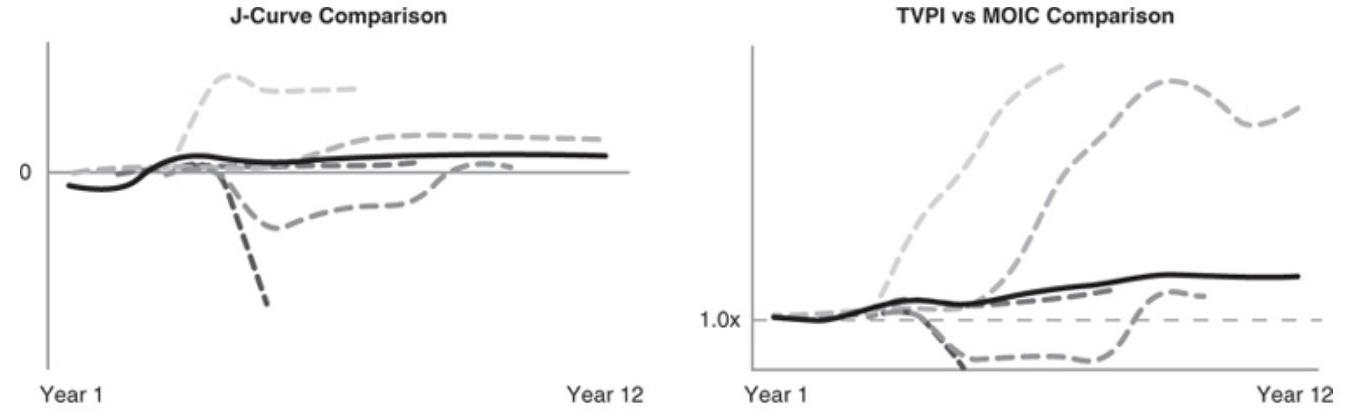
\includegraphics[max width=\textwidth, center]{2024_04_10_6394ed7f28ddb869f41dg-3(1)}\\
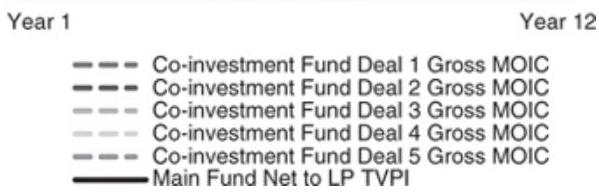
\includegraphics[max width=\textwidth, center]{2024_04_10_6394ed7f28ddb869f41dg-3}

Range of Outcome for Co-Investments Main Fund Net to LP IRR

Notes: Main fund return is net of fees, expenses, and carried interest. MOIC and TVPI are cumulative distributions and current net asset value (TVPI) or market value (MOIC) divided by cumulative paid-in or invested capital.

Source: Cambridge Associates (2015). "Making waves: The cresting co-investment opportunity.” Data from Cambridge Associates LLC Private Investments Database.


\end{document}